\section{大学におけるソフトウェア開発実習の制約と制約に対する対処}

本節では,大学においてソフトウェア開発実習を行う際に考慮しなければならない制約について述べる.

考慮する必要がある点は大きく分けて以下の3点である.

\begin{itemize}
\item[・] アジャイルソフトウェア開発手法で求められるソフトウェア開発のスキル
\item[・] アジャイルソフトウェア開発における開発チームと受講生間のプログラミングのレベル差
\item[・] アジャイルソフトウェア開発のための環境
\end{itemize}

\subsection{アジャイルソフトウェア開発手法で求められるソフトウェア開発のスキル}

アジャイルソフトウェア開発手法を実践するには,前章で述べたようなことができる,または前節で述べたようなツールを使える必要がある.

つまり

\begin{itemize}
\item[・]問題点や要求を分析しソフトウェアの変更点に落としこめる
\item[・]ソフトウェアの変更点に対してのテストコードを書ける
\item[・]アプリケーションフレームワークを利用しプロダクトコードが書ける
\item[・]バージョン管理システムを利用してコードを管理できる
\item[・]継続的インテグレーションシステムを利用し,ソフトウェアの品質を保つことが出来る
\end{itemize}

上記のような事が求められる.

しかし,上記のスキルはソフトウェア開発に置いて必要なことであり,コンピューターサイエンスとして必須では無いことから,これらのスキルを身につけるための授業が設置してあるとは考えづらい.特にアプリケーションフレームワークを利用することは,対象のプログラミング言語に対しての最低限の理解\footnote{例えば,クラスベースのオブジェクト指向プログラミングをサポートしているプログラミング言語ならば,クラスの記述方法や拡張方法,クラスから生成したインスタンスの利用方法などがあげられる}が必要となる.またWebアプリケーションのためのフレームワークならば,Web技術\footnote{Web技術とはHTMLやCSS,URLとプログラムの関係性やセッション,クッキーなどのこと}に対しての理解が必要となる.よって本研究で提案する授業はこれらの技術を習得もしくは理解していることを前提とする.


\subsection{受講生間のプログラミングのレベルの差}

アジャイルソフトウェア開発におけるチームメンバーは,自立的かつ自己組織的なメンバーが求められる.大学での授業であるという制約を考えなければ,ソフトウェア開発実習でもチームを編成し授業を実施するのが良いだろう.
しかし,ソフトウェア開発実習を受講する学生のプログラミングのレベルの差があり,もしグループワークでの授業を実施すると,グループの間のプログラミングができる人とできない人の間に割り振られるタスクの量と質に差がでる.タスクの割り振りによって,受講者が経験することが異なるのは避けたい.

この問題に対しては,授業の目標が「アジャイルソフトウェア開発に参加できるようになる」であることも考慮し,グループワークを採用せず,開発は参加者が各々に取り組む形を取るようにする.

\subsection{アジャイルソフトウェア開発のための環境}

本来であれば,使用するツールや開発フローは出来る限り,企業が使用しているものに近づけたい.
しかし,環境の構築には,そのための知識を要求したり,正しく動作するかの検証が必要なために手間がかかる.
本研究で提案する授業で集中したいことは,ソフトウェア開発に必要な手法やプログラミングを学ぶことであり環境を用意することではないので,サービスを利用する,ツールを用いる,学習の用途として不要な箇所は簡略化することが解決策として挙げることができる.

開発環境の用意に関しては,Vagrant (図?)と言うツールを用いて,予め利用する用意された仮想マシンのイメージを配布し,それを利用してもらうことで開発環境を用意する手間を省く.

実行環境としてはHerokuというPaaS\footnote{Platform as a Service の略}を用いる.Heroku (図)はWebアプリケーションと呼ばれるソフトウェアを実行する際に管理する必要のある,Webサーバー,アプリケーションサーバー,RDBMS,DNSなど自分のプログラム以外のほぼ全てを管理してくれるサービスである.

コードホスティングサーバーとして利用するサービスはGitHub (図?)を利用し,継続的インテグレーションツールとしてはCircleCI (図?)というSaaS\footnote{Software as a Serviceの略}を用いる.

\begin{figure}[H]
\centering
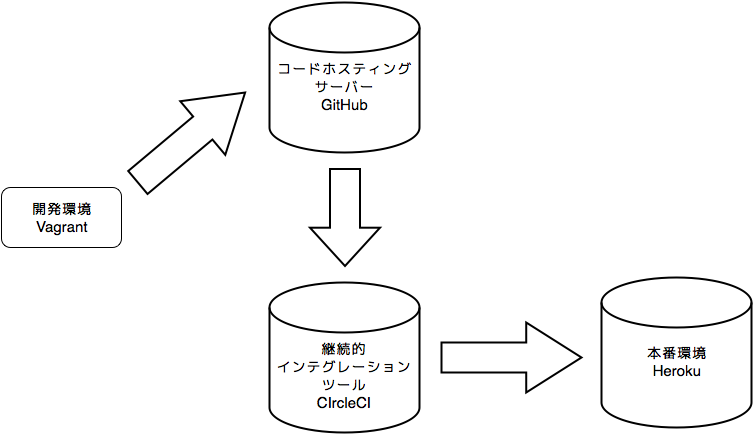
\includegraphics[height=8cm]{./assets/images/class_dev_env.png}
\caption{授業で用いる開発の環境概要図}
\label{fig:class_dev_env}
\end{figure}
